\documentclass[10pt,a4paper]{article}
\usepackage[utf8]{inputenc}
\usepackage{amsmath}
\usepackage{amsfonts}
\usepackage{amssymb}
\usepackage{natbib}
\usepackage{graphicx}

\title{Perceptron model theory}
\author{Max Cotton}
\date{}

\begin{document}

\maketitle

\section{Setup}

\begin{figure}[h!]
\centering
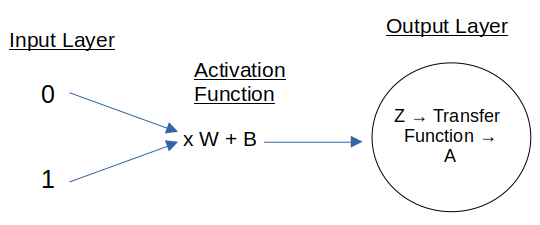
\includegraphics[width=1\textwidth]{src/utils/images/perceptron-ann-diagram.png}
\caption{This model uses no hidden layers and is known as a Perceptron Artificial Neural Netwok.}
\end{figure}

\begin{itemize}
    \item Where W is the array of weights, initially set to zeroes, and B is the array of biases, initially set to zeros
    \item Z is the dot product of the W array and the input array (X) summed with the B array
    \item A is sigmoid(Z), which is the prediction
    \begin{itemize}
        \item Where $sigmoid(Z) = \frac{1}{1+e^{-Z}}$
    \end{itemize}
\end{itemize}

\section{Forward Propagation}
For each epoch the input array of values, is fed through the network to obtain a prediction A

\section{Back Propagation}

\begin{itemize}
    \item Once a prediction is obtained, you then move back through the network adjusting the weights and the bias
    \item The "Loss" (L) (how wrong the prediction is) can be calculated with the Loss function, which calculates the average difference between the prediction and the actual value (Y), the average is found by summing the result for each prediction then dividing by the number of predictions (m). This shows how well the network is performing.
    \begin{itemize}
        \item Where $L = -(\frac{1}{m}) * \sum(Y * log(A) + (1-Y) * log(1-A))$ and "log()" is the natural logarithm (e is the base)
    \end{itemize}
    \item The weights and the bias are adjusted via Gradient Descent, which aims to get the minimum Loss value, with the following formulae:
    \begin{itemize}
        \item $W = W - learningRate * \frac{\partial{L}}{\partial{W}}$
        \begin{itemize}
            \item Where $\frac{\partial{L}}{\partial{W}} = X * (\frac{1}{m})(A-Y)$
        \end{itemize}
        \item $B = B - learningRate * \frac{\partial{L}}{\partial{B}}$
        \begin{itemize}
            \item Where $\frac{\partial{L}}{\partial{B}} = (\frac{1}{m})(A-Y)$
        \end{itemize}
    \end{itemize}
\end{itemize}

\section{Derivations for $\frac{\partial{L}}{\partial{W}}$ and $\frac{\partial{L}}{\partial{B}}$}

\begin{itemize}
    \item Functions used so far:
    \begin{enumerate}
        \item $Z = W . X + B$
        \item $A = \frac{1}{1+e^{-Z}}$
        \item $L = -(\frac{1}{m}) * \sum(Y * log(A) + (1-Y) * log(1-A))$
    \end{enumerate}
    \item $\frac{\partial{L}}{\partial{W}}$ derivation:
    \begin{itemize}
        \item By the Chain rule, $\frac{\partial{L}}{\partial{W}} = \frac{\partial{L}}{\partial{A}} * \frac{\partial{A}}{\partial{Z}} * \frac{\partial{Z}}{\partial{W}}$
        \item Using function 3, $\frac{\partial{L}}{\partial{A}} = (-\frac{1}{m})(\frac{Y-A}{A * (1-A)})$
        \item Using function 2, $\frac{\partial{A}}{\partial{Z}} = A * (1-A)$
        \item Using function 1, $\frac{\partial{Z}}{\partial{W}} = X$
        \item => $\frac{\partial{L}}{\partial{W}} = (-\frac{1}{m})(\frac{Y-A}{A * (1-A)}) * A * (1-A) * X\\
              = X * (\frac{1}{m})(A-Y)$
    \end{itemize}
    \item $\frac{\partial{L}}{\partial{B}}$ derivation:
    \begin{itemize}
        \item By the Chain rule, $\frac{\partial{L}}{\partial{B}} = \frac{\partial{L}}{\partial{A}} * \frac{\partial{A}}{\partial{Z}} * \frac{\partial{Z}}{\partial{B}}$
        \item Derived above, $\frac{\partial{L}}{\partial{A}} = (-\frac{1}{m})(\frac{Y-A}{A * (1-A)})$
        \item Derived above, $\frac{\partial{A}}{\partial{Z}} = A * (1-A)$
        \item Using function 1, $\frac{\partial{Z}}{\partial{B}} = 1$
        \item => $\frac{\partial{L}}{\partial{W}} = (-\frac{1}{m})(\frac{Y-A}{A * (1-A)}) * A * (1-A)\\
              = (\frac{1}{m})(A-Y)$
    \end{itemize}
\end{itemize}

\end{document}